% chktex-file 46
%!TeX spellcheck = en-US,it-IT
\chapter{The Problem}

The scope of this thesis is considering a classic signal-background
discrimination task by following the path outlined by~\cite{paper}
and~\cite{gaia} to find a reasonably good machine learning classifier built
on top of a Deep Neural Network model. The intention is to use the results
in the just cited works to fix some hyper-parameters and reduce our degrees
of freedom. Then to develop a program to explore the time
performance in training such models using clustering and GPU (graphics
processing unit) architectures.

\section{Deep Neural Networks}

Machine Learning (ML) is a field of artificial intelligence that uses
statistical techniques to give computer system the ability to learn from
data without being explicitly programmed.~\cite{ML} One example of machine learning
task is the classification problem. You have, for instance, a dataset with
many records. Each of them composed of some features that
describe it and one label that indicates in which class among two or more
the record belong. Using these information, in the training phase, the
ML model learns to classificate the records in the correct class. After the
training phase, there is a test one when the classifier performance is been
tested with unseen records.

Deep Learning is a sub-field of Machine Learning that deals with algorithms
inspired by the structure and function of the brain called deep neural
networks (DNNs).
More concretely a neural network is a function
$f\colon\mathbb{R}^n\to\mathbb{R}^m$ from the space of the features to the
space of the labels. It is structured in layers and consist of an input
layer of size $n$, an output layer of size $m$ and several hidden layers
of various sizes. Each element of layers is called neuron and each neuron
is connected with all previous layer neurons and with all those of the
next (Figure~\ref{nns}).
\begin{figure}[htpb]
 %\begin{wrapfigure}{r}{0.33\textwidth} %this figure will be at the right
 \centering
 %    \includegraphics[width=0.25\textwidth]{mesh}
 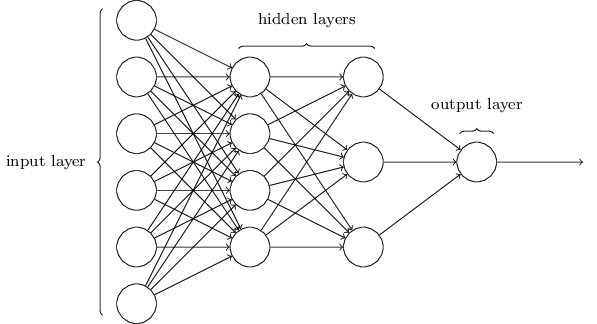
\includegraphics[scale=0.55]{figures/nnstructure.png}
 \caption{Neural Network structure}
 \label{nns}
 %\end{wrapfigure}
\end{figure}
These connections are mathematically described by weights, such as the input
of a neuron is determined by
\[
 y_i = \mathbf{w}_i \cdot \mathbf{x} + b_i = \sum_{j=1}^{q}w_{ij}x_j + b_i
\]
where $\mathbf{x}$ is the input values vector or the outcome of the
previous layer, $\mathbf{w}_i$ is instead the weight vector that corresponds
to the $i$-th neuron. A function $h$ is then applied to each of the $i$
neurons, it is called layer \textit{activation function} and it
yields as an output $\mathbf{z}=\{ z_i = h(y_i)\colon i = 1,\ldots,q\}$. This
process is being repeated through the network until the output layer is
reached.
There are some options for initializing weights
\begin{itemize}
 \item all initialized to a fixed value
 \item campionated from standard gaussian distribution
 \item campionated from uniform distribution
 \item other distributions
 \item etc.
\end{itemize}
it has been chosen to campionate them from a standard gaussian distribution.

The next step is understand how well the model predicts labels from data.
To achieve this we choose a \textit{loss function} that has the
characteristic to become smaller and smaller as the model learn, \eg~
perform better. Hence, the job is minimizing this function. In order to achieve
it several optimizing algorithms, or optimizers, exist.
The description of (some of these/the smoothest one: sgd) is given in
the next section.

Had obtained the neural network model, it is remarkable to note that there
is a theorem that states~\cite{theorem}
\begin{teorema}
 Feedforward networks are capable of arbitrarily accurate approximation
 to any real-valued continuous function over a compact set.
\end{teorema}

This is clearly excellent for us. Despite the fact that under certain
hypothesis almost every function can be represented by a neural network,
the maximum complexity achievable, however, depend on the choice of some of the
hyperparameters. Such as the number of layers, the number of neurons
for layer and the activation functions. A bad choice of these
hyper-parameters leads to a poor model that can not generalize well the problem
(underfitting) or a too complex model that does not fit well (overfitting).
On the other hand, the learning process itself must be
performed taking into account a series of issues that can lead to
underfitting or overfitting. Refer to~\cite{deeplearningbook} regarding
this (vast) topic.
\subsection{SGD}
The algorithm. A brief derivation. Some formulas.


\subsection{others..?}
Same.

\section{the physics of LHC}

The \textit{European Organization for Nuclear Research}, known as
\textit{CERN}, is a European research organization that operates the
largest particle physics laboratory in the world. \textit{CERN} is the
host of the \textit{Large Hadron Collider} (\textit{LHC}), the largest
particle accelerator in the world. Along its circumference four detectors
are arranged. \textit{CMS}, \textit{ATLAS} and \textit{LHCb} detect only
proton-proton collisions while \textit{ALICE} is used with collisions
between lead ions too. These four experiments carried on at \textit{LHC}
detect a great number of hadrons collisions per second and for each event
are record various forms of data. The large size, the variety and the high
rate of collisions production at \textit{LHC} are the reasons are named
\textit{big data} and these are one of the most suitable dataset for
testing efficiency of Neural Networks techniques. On the other hand,
employing more and more efficient machine learning algorithms to
\textit{LHC} datasets will let high energy physics community to extract
from data more information. This would reduce the waste of data.

\begin{figure}[htpb]
 \centering
 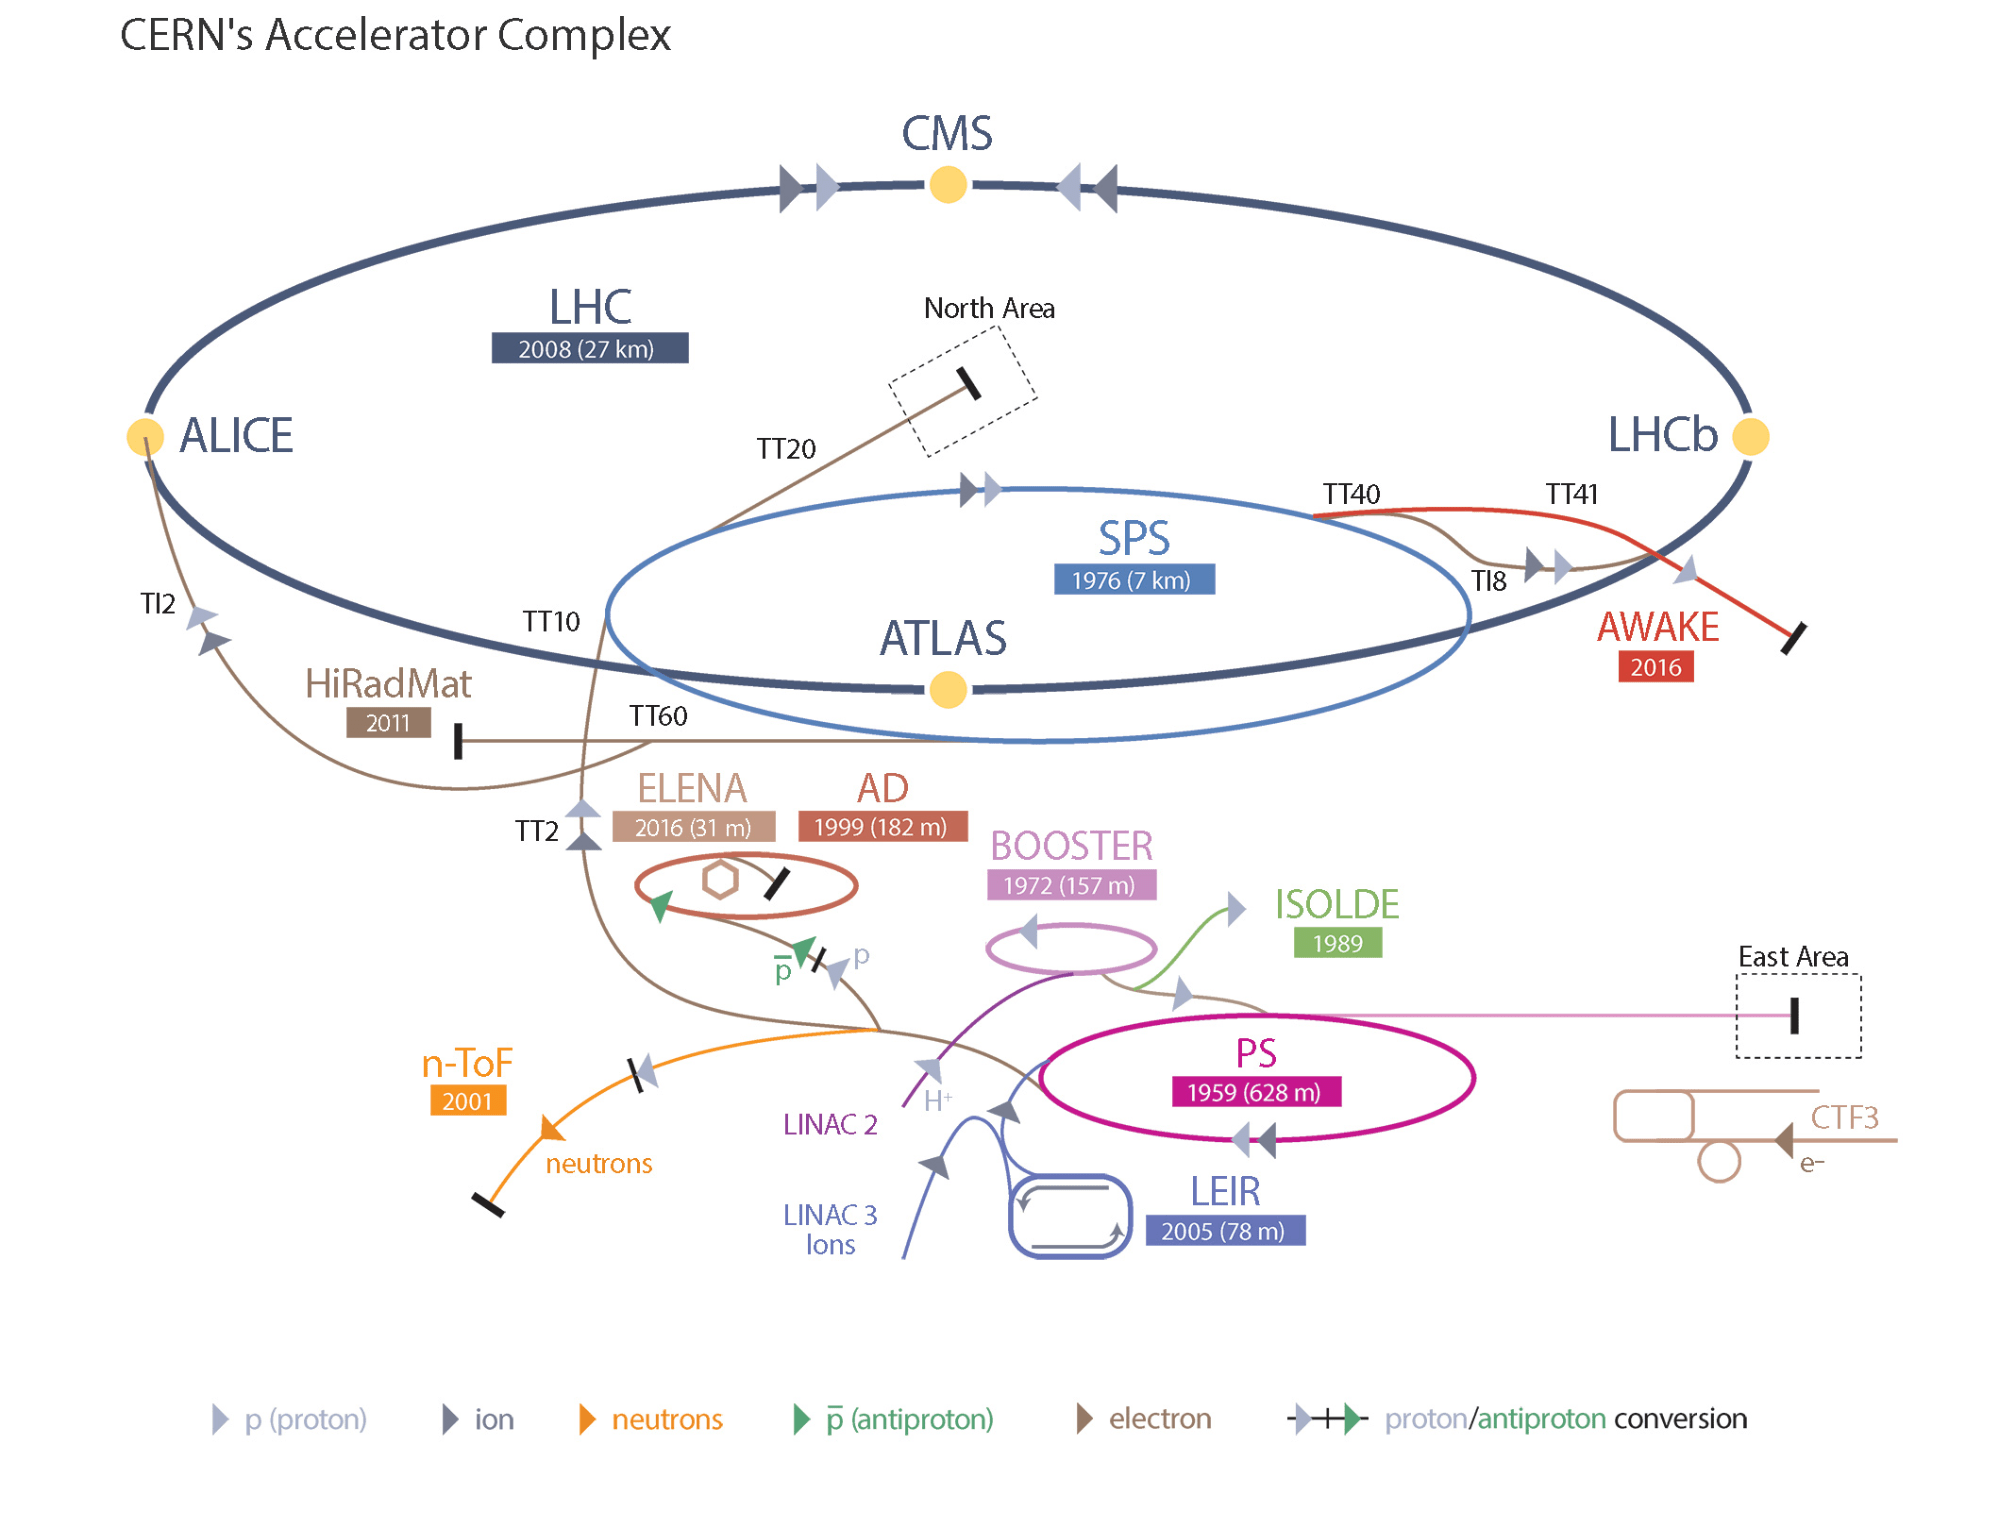
\includegraphics[scale=0.18]{figures/lhc2.png}
 \caption{\textit{LHC} complex}
 \label{}
\end{figure}

The \textit{LHC} accelerator itself consists of a $27$-kilometer ring of
superconducting magnets with a number of accelerating cavities to make
beams focused in order to maximize the cross section. Also for curve the
trajectory and increase the energy of the particles circulating inside its
rings. The preparatory phase pf acceleration begin at the Linac 2 where the
protons from hydrogen are accelerated to $50$ MeV. The beam is then get
injected into the Proton Synchrotron Booster (PSB) where the proton bunches
are formed and accelerated further to $1.4$ GeV. The next accelerator is
called the Proton Synchrotron (PS) which forms the final shape of the beam
bunches and kicks the beam up to $25$ GeV. The particles are later sent to
the Super Proton Synchrotron (SPS) where they are accelerated to $450$ Gev,
from which they are injected into two pipes of the \textit{LHC}. This is
where the beams go in opposite directions to be collided at the
experimental sites with up to a center-of-mass energy of $\sqrt{s}=14$ TeV.

Taking the CMS detector as an example it is formed by a series of cylindrical
sub-detectors able to detect different interactions. This for the purpose
of study many aspects of the high energy interactions between protons, from
the Standard model parameters to the New Physics theories and their
associated particles. Different technologies are used to observe different
features of the particles going across them. The closest one is a vertex
detector of silicon pixels and strips used to track charged particles near
to the point of interaction. Then there is the charged particle tracking
chamber which distinguishes positive and negative charges measuring the
curvature of the particles in a magnetic field. Next layer consists in two
calorimeters: one absorbing the electromagnetic-showers and the other the
hadronic-showers. Finally, the muon chambers which absorb the heaviest
particles called muons. All these components together are able to absorb
all the energy issued by the collision except that carried out by
neutrinos. From the pieces of information collected by each layer of the
detector, high energy physicists are able to go back to the nature of the
particles produced by the collision and study the laws which regulate these
processes.

\begin{figure}[H]
 \centering
 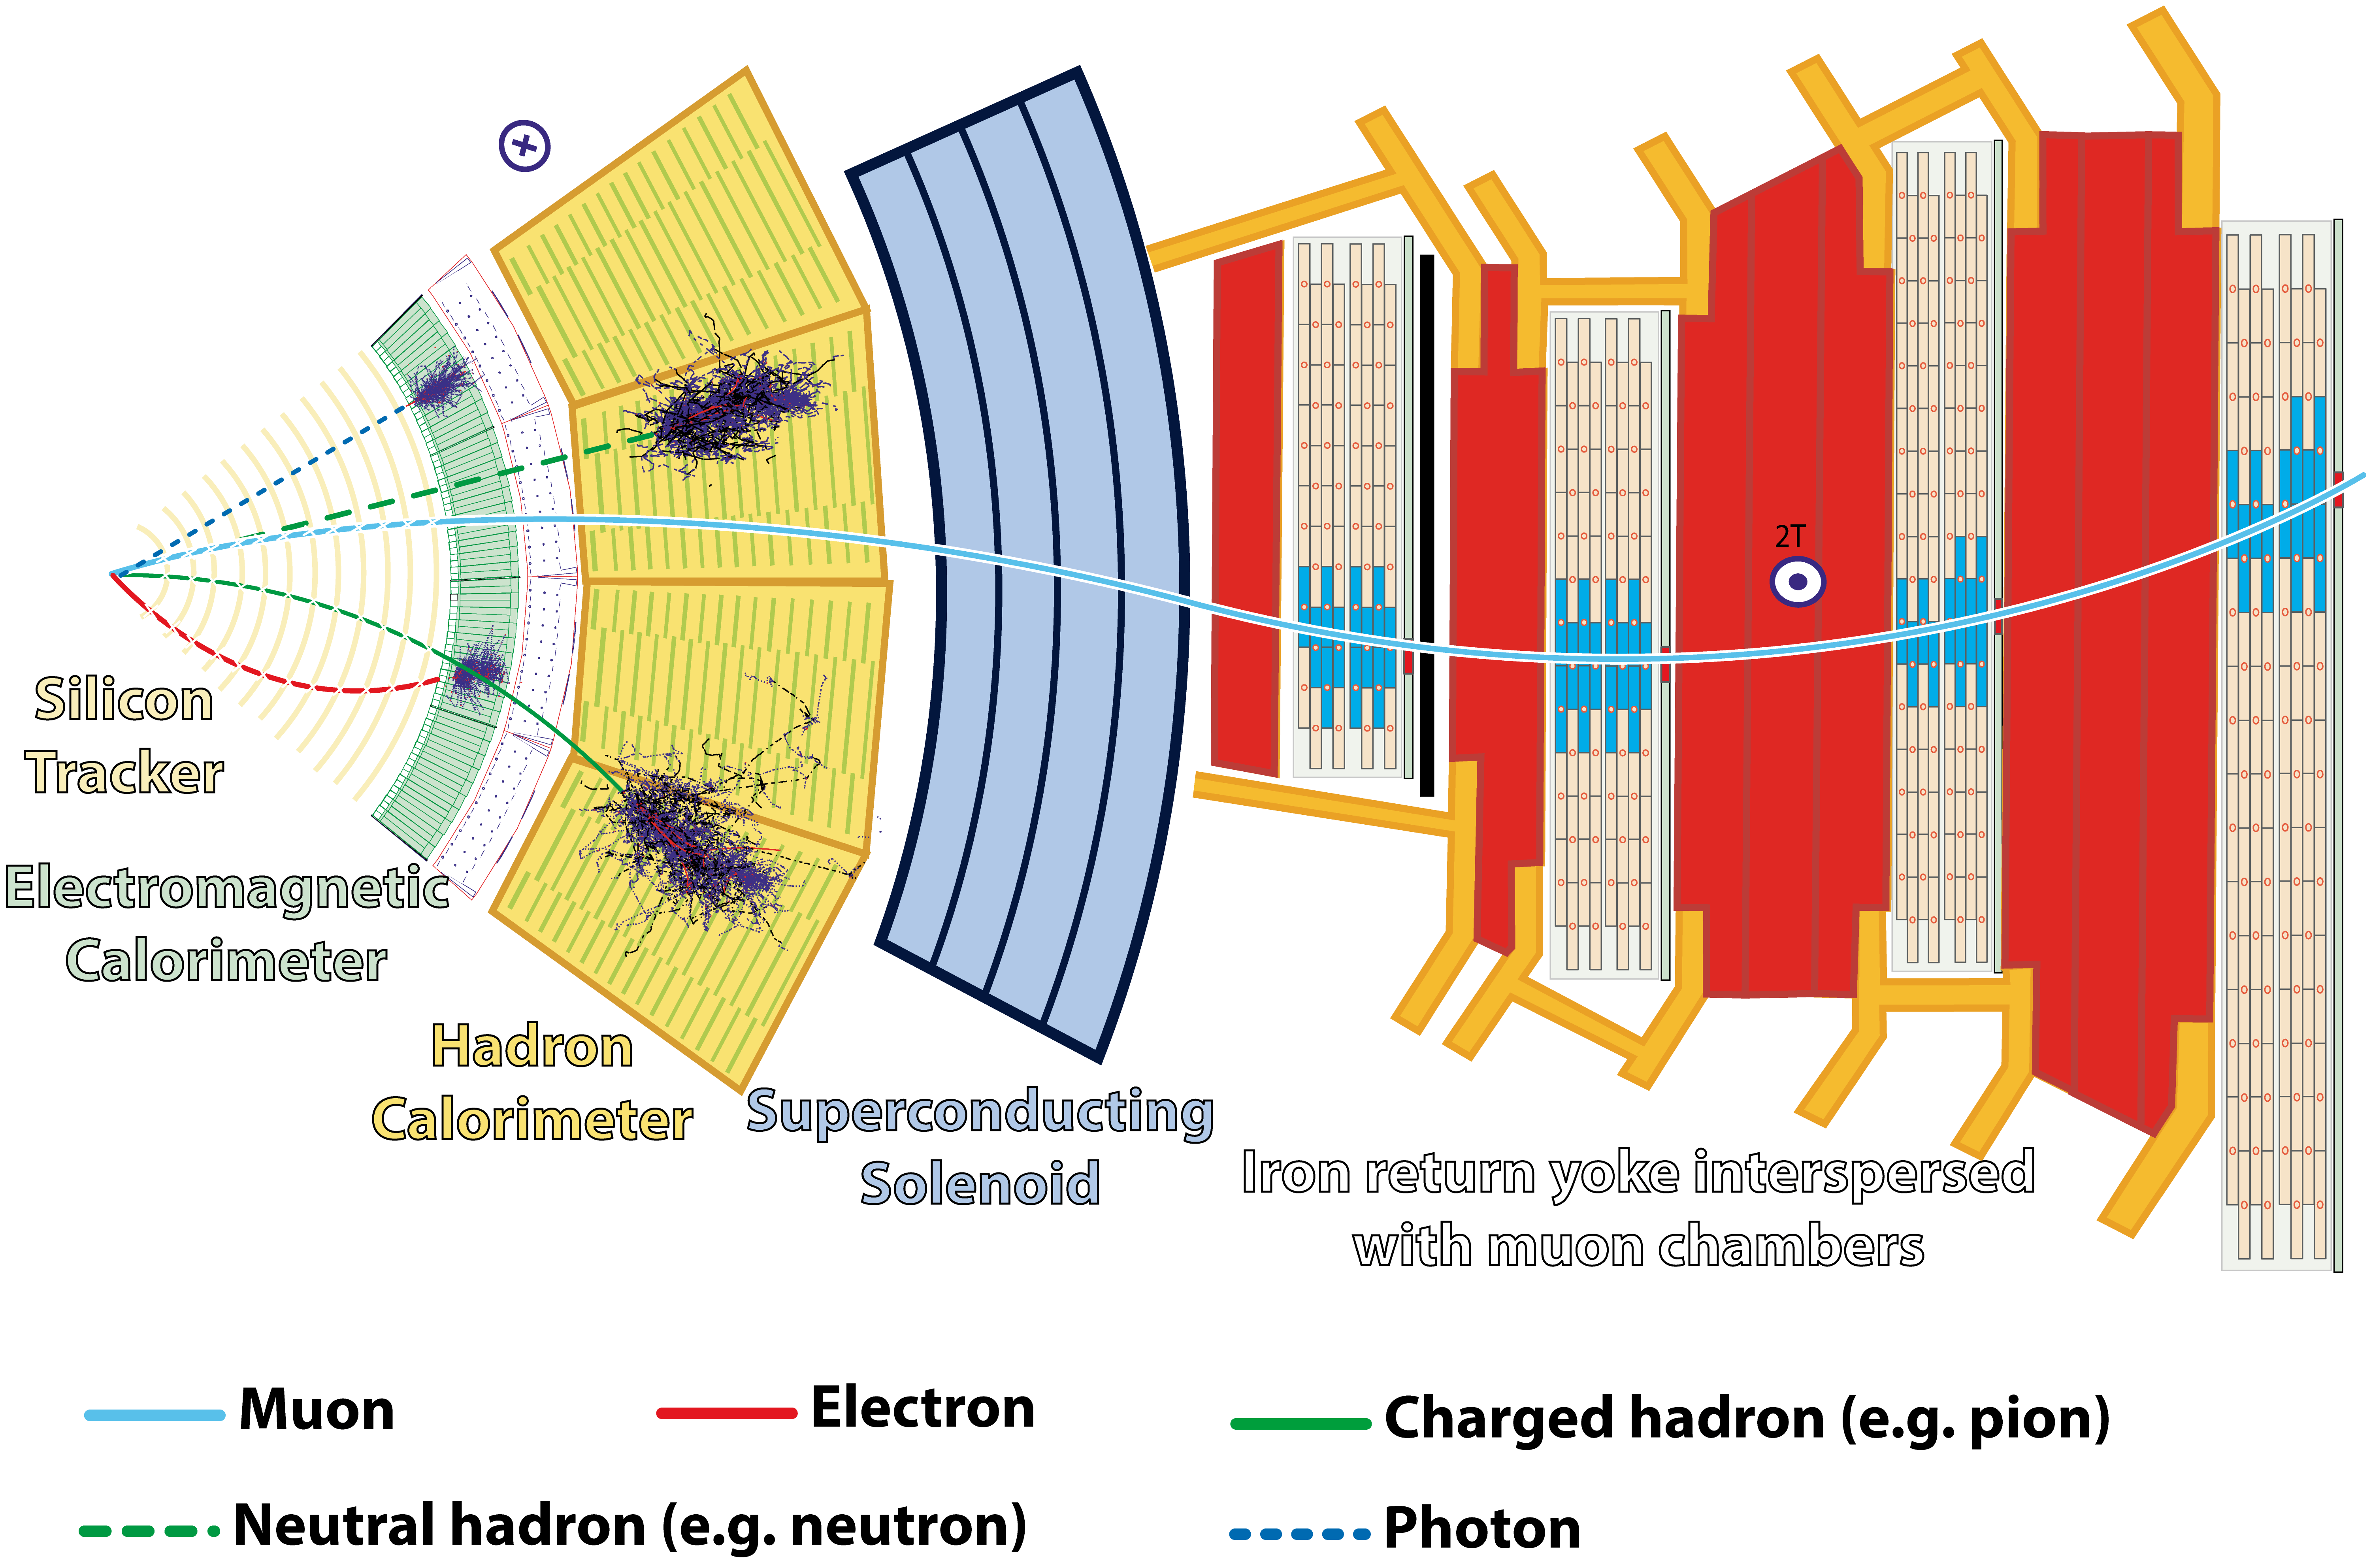
\includegraphics[scale=0.05]{figures/CMSslice.png}
 \caption{A transverse section of the CMS detector}
 \label{}
\end{figure}

\section{The benchmark dataset HIGGS}\label{data}%\footnote{The features
% distribution are in the Appendix}
The dataset subject of this work involves a signal process where new Higgs
bosons are produced and a background process with identical decay products
but distinct kinematic features.
The signal process is the fusion of two gluons into a heavy
electrically-neutral Higgs boson ($gg \rightarrow H^0$), which decays
to a heavy electrically-charged Higgs boson ($H^\pm$) and a $W$ boson.
The $H^\pm$ subsequently decays to a second $W$ boson and in a light Higgs
boson, $h^0$. The light Higgs boson then decays predominantly to a pair of
bottom quarks. The entire process is then:
\begin{equation}
 gg \rightarrow H^0 \rightarrow W^\mp H^\pm \rightarrow W^\mp W^\pm h^0
 \rightarrow W^\mp W^\pm b \bar{b}
\end{equation}
which leads to $W^\mp W^\pm b \bar{b}$. The background process, which
mimics $W^\mp W^\pm b \bar{b}$ without the Higgs boson intermediate state
is the production of a pair of top quarks, each of which decays to $Wb$
(see figure 1.):
\begin{equation}
 gg \rightarrow g \rightarrow t\bar{t} \rightarrow W^\mp W^\pm b \bar{b}
\end{equation}

\begin{figure}[htpb]
 \centering
 \subfloat[][]{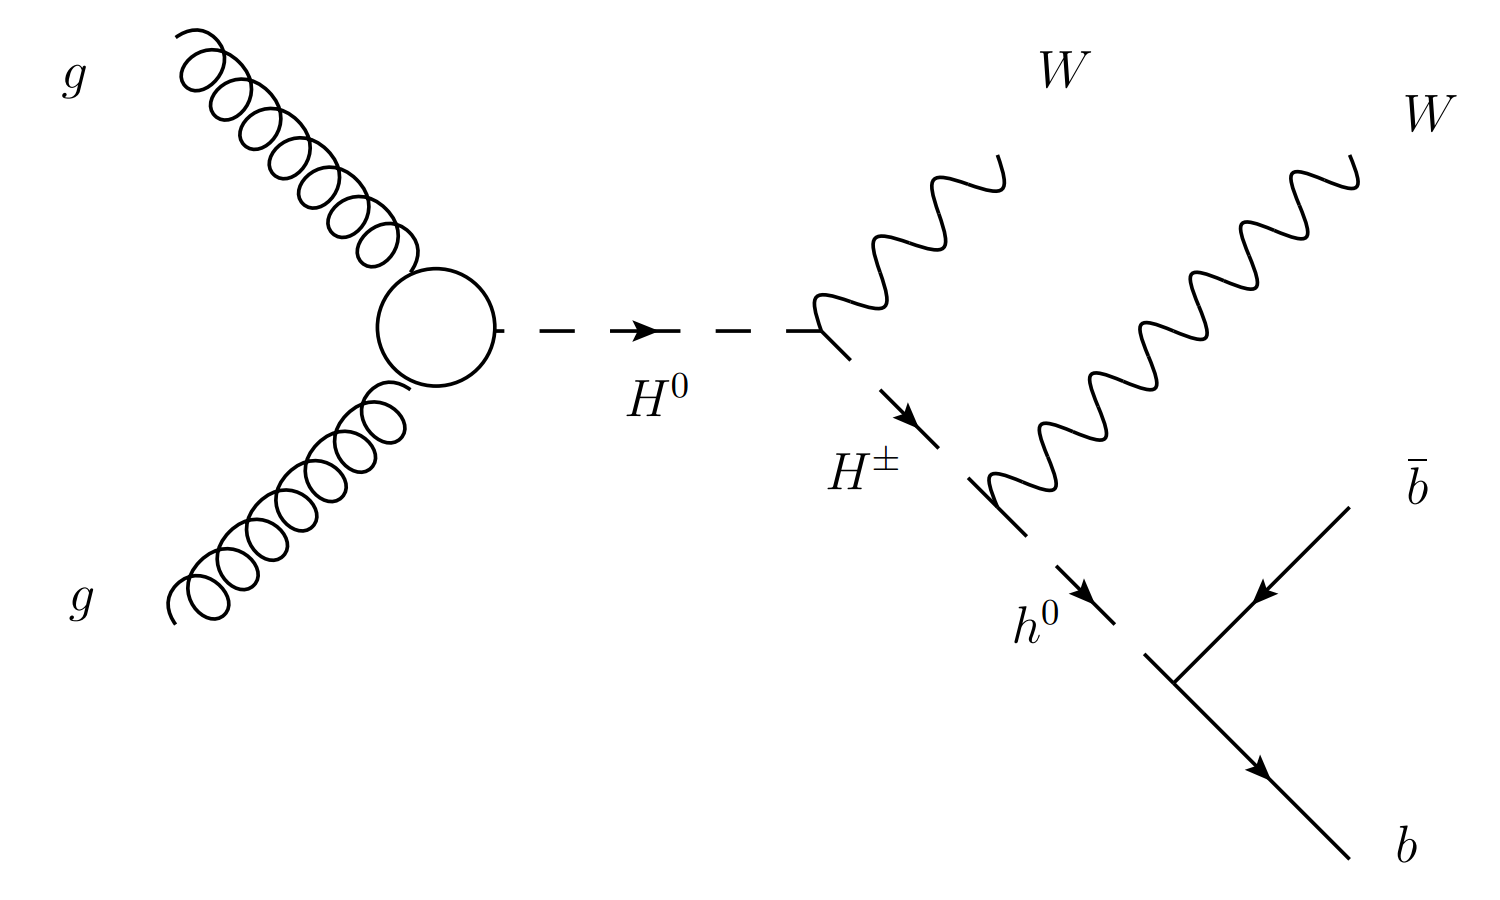
\includegraphics[width=.45\textwidth]{figures/decs.png}} \quad
 \subfloat[][]{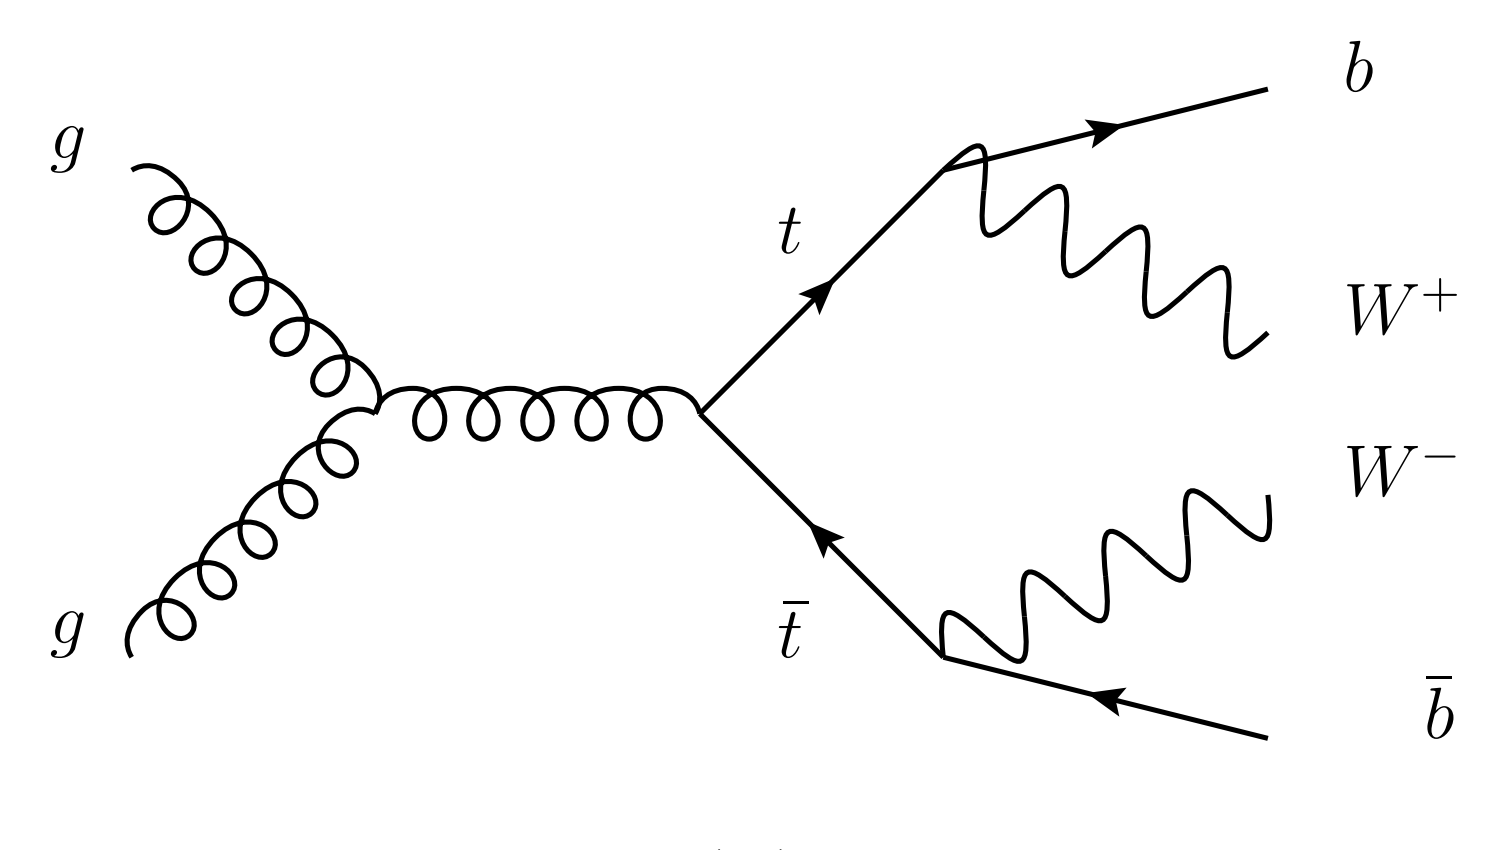
\includegraphics[width=.45\textwidth]{figures/decb.png}} \\
 \caption{(a) Diagram describing the signal process involving new exotic
  Higgs bosons $H^0$ and $H^\pm$. (b) Diagram describing the background
  process involving top-quarks ($t$). In both cases, the resulting
  particles are two $W$ bosons and two $b$-quarks.}
 \label{graphs}
\end{figure}

accordingly, to~\cite{paper} the events are simulated assuming $8$ TeV
collisions of protons at LHC. For the benchmark case here, $m_{h^0}=125$
GeV, $m_{H^0}=425$ GeV and $m_{H^\pm}=325$ GeV has been assumed.
In order to simulate events for this dataset the semi-leptonic decay mode has
been chosen, which is one $W$ boson decaying to a lepton and a
neutrino($l\nu$) and the other $W$ boson in a pair of jets (which
correspond to a couple of up-type and down-type quarks). Thus, the
final products of our decays are $l\nu b j j  b$.
In \cite{paper} has been considered events which satisfy (and we do
accordingly):
\begin{itemize}
 \item exactly one electron or muon, with $p_T > 20$ GeV and
       $\vert \eta \lvert < 2.5$
 \item at least four jets, each with $p_T > 20$ GeV and
       $\vert \eta \lvert < 2.5$
 \item $b$-tags on at least two of the jets, indicating that they are
       likely due to $b$-quarks rather than gluons or lighter quarks
\end{itemize}

where $p_T$ is the momentum transverse to the beam direction and
(referred to a polar coordinate system) the polar angle $\theta$
is substituted by
\[
 \eta = -\ln{\tg{\frac{\theta}{2}}}
\]
there is then the azimuthal angle $\phi$.
The above requirements are then summed up by 21 low-level features:
\begin{itemize}
 \item $4$ jets, each of them described through $4$ variables: $p_T$,
       $\eta$, $\phi$ and the $b$-tag.
 \item $1$ lepton described through 3 variables: $p_T$, $\eta$, $\phi$
 \item $1$ neutrino indirectly described by: missing energy magnitude and
       missing energy $\phi$
\end{itemize}

Theoretical considerations allow constructing new high level features
which better highlight the differences between these two processes.
The features are the invariant masses of the metastable particles.
In particular, for signal processes the following resonant decays have
been theorized and the related invariant masses have been computed:
\begin{itemize}
 \item $W \rightarrow l \nu$: the invariant mass $m_{l\nu}$ should show
       in the known mass of the $W$ boson $m_W$
 \item $W \rightarrow jj$: the invariant mass $m_{jj}$ should show a peak
       at the known mass of the $W$ boson $m_W$
 \item $h^0 \rightarrow b\bar{b}$: $m_{b\bar{b}}$ should show a peak at
       $m_{h^0}$
 \item $H^\pm \rightarrow W^\pm h^0$: $m_{Wbb}$ should show a peak at
       $m_{H^\pm}$
 \item $H^0 \rightarrow WH^\pm$: $m_{WWb\bar{b}}$ should show a peak at
       $m_{H^0}$
\end{itemize}
there represent $5$ high-level features. On the other hand,
regarding $t\bar{t}$ background, it is expected that:
\begin{itemize}
 \item $W \rightarrow l \nu$ shows a peak in $m_{l\nu}$ at $m_W$
 \item $W \rightarrow jj$ shows a peak in $m_{jj}$ at $m_W$
 \item $t \rightarrow Wb$ shows a peak in $m_{jl\nu}$ and $m_{jb\bar{b}}$ at
       $m_t$
\end{itemize}
thus two more invariant masses $m_{l\nu b}$ and $m_{jjb}$ have been
computed. In total there are 7 high-level features. Before being passed to
the neural networks the dataset had been standardized removing mean and
standard deviation from features. The just described sample with 11 million
events is available in the UCI machine learning
repository.\footnote{https://archive.ics.uci.edu/ml/datasets/HIGGS}


\section{The setup (bigdl?)}

The used hardware is composed by a six nodes (computers) cluster hosted by
Cloudveneto\footnote{https://cloudveneto.ict.unipd.it/} and a GPU machine
under the same domain. In a cluster, one node is called cluster manager or
master, while the others workers or slaves.
In this case, the master is a computer with $2$ cores and
$\SI{4}{\giga\byte}$ of RAM while the $5$ nodes are computers with $8$
cores and $\SI{16}{\giga\byte}$ of RAM, for a total of $40$ cores and
$\SI{80}{\giga\byte}$ of RAM for the slaves.
The master role is to dispatch individual small tasks to the slaves that
send back the processed results. This paradigm is carried out by Apache
Spark\cite{spark} which is a \textit{unified analytics engine for large-scale
 data processing}\footnote{https://spark.apache.org/}.
Spark applications run as independent sets of processes coordinated by the
\lstinline{SparkContext}
object in the main program (\textit{driver program}).
Specifically, to run on a cluster, the SparkContext connect
to a \textit{cluster manager} which allocate resources across applications.
Once connected, Spark acquires \textit{executors} on nodes in the cluster,
which are the processes that run computations and store data to process.
Next, it sends the application code to the executors. Finally, SparkContext
sends \textit{tasks} to the executors to run.
\begin{figure}[htpb]
 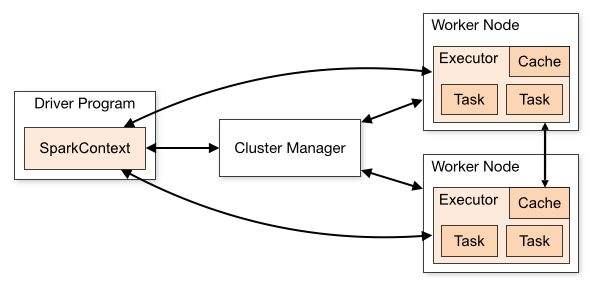
\includegraphics[scale=0.55]{figures/cluster-overview.png}
 \caption{The Spark architecture}
 \label{}
\end{figure}

The driver program has been written in Python\footnote{https://www.python.org/}
which is a high level programming language widely used nowadays for data
science topics. In the program, through Spark application program interface
(API), instructions are sent to workers. Spark use as backend Java, meaning
that the execution of the Spark code is committed to a Java interpreter which
is a lower level programming language. This is a common programming paradigm,
the code is written in a higher level language while the actual execution is
performed by a lower one. Python itself is written in \CC~which is one of the
oldest and still very used low level programming language.

While the framework used is Spark, the utilized library for implementing the
distributed Deep Neural Network models is BigDL~\cite{bigdl} from Intel
Corporation. Instead, for the standalone and the GPU version has been used
Keras~\cite{keras} with Tensoflow~\cite{tensorflow} backend.

The work done in~\cite{gaia} and~\cite{paper} has been used for fix some
hyperparameters:
\begin{itemize}
 \item Number of layers: $3$
 \item Neuron for layer: $300$
 \item Dropout: $0$
 \item Layer activation function: \textit{tanh}
 \item Output activation function: \textit{sigmoid}
 \item Learning Rate: Default value of the optimizer
\end{itemize}

For what concern the hidden layers activation function the
$tanh$ function has been chosen. Instead, for the output neuron a sigmoid
has been taken.
\begin{figure}[h]
 \begin{minipage}{.5\textwidth}
  \begin{equation*}
   \tanh(x) = \frac{\me^x-\me^{-x}}{\me^x+\me^{-x}}
  \end{equation*}
  \begin{equation*}
   \text{sig}(x)=\frac{1}{1+\me^{-x}}
  \end{equation*}
 \end{minipage}%
 \begin{minipage}{.5\textwidth}
  \centering
  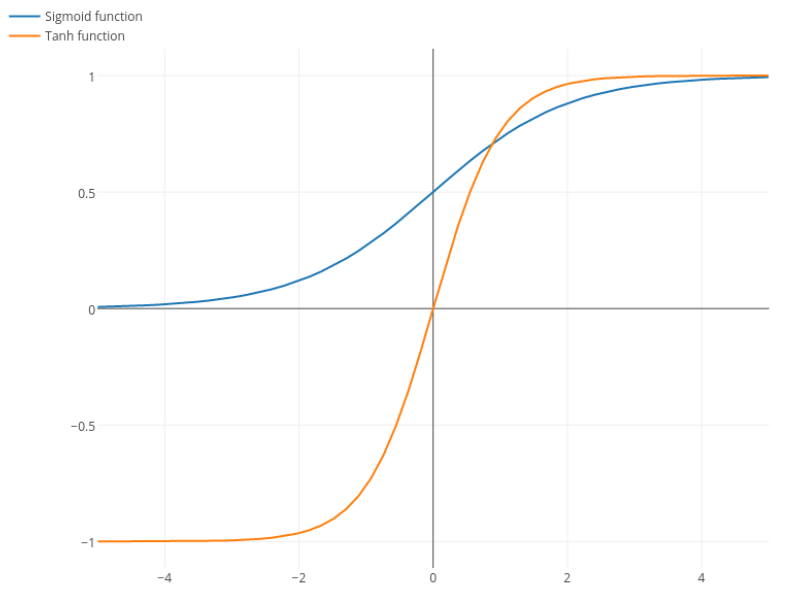
\includegraphics[scale=0.3]{figures/SeT.png}
 \end{minipage}
 \caption{tanh and sigmoid functions comparison}
\end{figure}

The sigmoid function has the property of returning an output in the interval
$\left(0,1\right)$ it can be seen as the confidence the network has
regarding the $0$ or the $1$ classification. It means that the closer to $1$
is the output the more confident the network is about the event
classification as a signal, vice versa a result near $0$ means a background
event. It is a very common choice for an output function for a Machine
Learning classifier.
